\section{可靠性数据与生存分析部分}\label{SecReliabilityAndSurvivalAnalysis}
\begin{center}
    Instructor: Jiangdian Wang 
\end{center}

Key focus of reliability data and survival analysis: Study the `survival time' $ T $ before some `failure event'. Basically the research problem is the distribution of $ T $, including topics on descriptive statistics, estimation and hypothesis testing. Further for actual cases, $ T $ might be censored, i.e. the observe time is not exact; and we may also wonder the influence of covariants $ z $.

\subsection{Reliability Data}
The main feature of reliability data is \textbf{censoring}, to be distinguished from the exact numbers in usual statistical inference. Censor means we cannot observe the exact \textbf{event time} $ T $. Instead, a \textbf{censoring time} $ C $ is observed, together with a censoring type, e.g. 
\begin{align}
    \text{Right Censoring: }&T_\mathrm{actual}>C \\
    \text{Left Censoring: }&T_{\mathrm{actual} }<C\\
    \text{Interval Censoring: }&C_l<T_{\mathrm{actual} }<C_r\\
    \cdots&
\end{align} 

\subsubsection{Right Censor Data and Representation}
\index{Censoring Data}
In most parts of this course we focus on right censor data, i.e. dataset contains both event time $ T $ and right censor time $ T^+ $:
\begin{align}
    \text{Event Time: }&T_1,\ldots,T_{n_1}\\
    \text{Right Censor: }&T^+_{1},\ldots ,T^+_{n_r}\\
\end{align}

Or we could use an indicator $ \delta  $ to express whether a time is event (1) or right censored (0):
\begin{equation}
    (T_i,\delta _i;z_i),\, i=1,2,\ldots n_1+n_r 
\end{equation}
where $ z_i $ for covariants.

Usually we assume that event and censor are independent $ T\independent C $

\subsubsection{Life Table Data}
Life table collect survival data at ordinal, uniformly-spaced time points, where each row contains \# items at risk, \# events, $ \ldots  $.


\subsection{Survival Model and Statistical Inference}
\subsubsection{Survival Function and Hazard}
Key focus of survival analysis problem is the distribution of $ T $ (note that in actual cases we need to make use of both event time $ T_i $ and censored data $ T^+_i $ to estimate the distribution of $ T $). The distribution feature can be described in various approaches: PDF $ f(t) $, CDF $ F(t) $, Survival Function $ S(t) $, Hazard Function $ \lambda (t) $, Cumulative Hazard Function $ \Lambda (t) $:
\begin{itemize}[topsep=2pt,itemsep=0pt]
    \item Continuous Case: $ t\in \mathbb{R}^+ $
    \begin{itemize}[topsep=2pt,itemsep=0pt]
        \item Survival Function $ S(t) $:\index{Survival Function}
        \begin{equation}
            S(t)\equiv 1-F(t) =\int _t^\infty f(\tau) \,\mathrm{d}\tau,\qquad f(t)=-\dfrac{\mathrm{d}^{} S(t)}{\mathrm{d}t^{}}
        \end{equation}
        
        \item Hazard Function $ \lambda (t) $ (or in some materials denoted $ h(t) $): mortality at $ t $:\index{Hazard Function}
        \begin{equation}
            \lambda (t)=\lim_{h\to 0}\dfrac{\mathbb{P}[t\leq T<t+h|T\geq t]}{h}= \dfrac{f(t)}{S(t)}=-\dfrac{\mathrm{d}^{} \log S(t)}{\mathrm{d}t^{}}
        \end{equation}
        \item Cumulative Hazard Function $ \Lambda (t) $ (or in some materials denoted $ H(t) $):
        \begin{equation}
            \Lambda (t)=\int _0^t \lambda (\tau) \,\mathrm{d}\tau =-\log S(t)
        \end{equation}
        \begin{equation}
            S(t)=e^{-\Lambda (t)}=e^{-\int _0^t \lambda (\tau) \,\mathrm{d}\tau} 
        \end{equation}
        
    \end{itemize}
    \item Discrete Case: $ t\in \{t_1,t_2,\ldots,t_n\} $
    \begin{itemize}[topsep=2pt,itemsep=0pt]
        \item PMF: $ p(t) $ is defined on 
        \begin{equation}
            t\in\mathcal{T},\quad p(t)\in (\mathcal{T}\to [0,1]^n]) 
        \end{equation}
        \item Survival Function: Note that CDF $ F(t) $ is right continuous, then $ S(t) =1-F(t)$ is left continuous:
        \begin{equation}
            S(t)=\mathbb{P}(T>t)=\sum_{t_i>t} p(t_i),\qquad p(t_i)=S(t_{i-1})-S(t_i)=\lambda (t_i)S(t_{i-1})
        \end{equation}
        
        Decomposition of survival function into hazard production
        \begin{align}\label{EqaSurvivalFunctionDecomposition}
            S(t)=&\mathbb{P}(T>t)=P(T>t\cap T>t_j),\quad \forall t_j<t\notag\\
            =&\mathbb{P}(T>t|T>t_j)\cdot \mathbb{P}(T>t_j)\notag\\
            =&\mathbb{P}(T>t|T>t_j)\cdot {\color{red} \mathbb{P}(T>t_j|T>t_{j-1})}\cdot \mathbb{P}(T>t_{j-1})\notag\\
            =&\mathbb{P}(T>t|T>t_j)\cdot {\color{red}\dfrac{S(t_j)}{S(t_{j-1})}}\cdot \mathbb{P}(T>t_{j-1})\notag\\
            =&\prod_{0<t_j\leq t}\dfrac{S(t_j)}{S(t_{j-1})}\notag\\
            =&\prod_{0<t_j\leq t}\left[ 1-\lambda (t_j) \right] 
        \end{align}

        \item Hazard Function $ \lambda (t) $:
        \begin{equation}
            \lambda (t_i)=\mathbb{P}(T=t_i|T\geq t_i)=\dfrac{p(t_i)}{S(t_{i-1})} =1-\dfrac{S(t_i)}{S(t_{i-1})}
        \end{equation}
        
        
        
    \end{itemize}
    
        
\end{itemize}


\begin{point}
    Properties of survival function and hazard function \& More concepts and definition
\end{point}

\begin{itemize}[topsep=2pt,itemsep=0pt]
    \item Mean Survival Time:
    \begin{equation}
        \mu \equiv\mathbb{E}(T)=\begin{cases}
            \int _{0}^\infty \tau f(\tau) \,\mathrm{d}\tau =\int _0^\infty S(\tau) \,\mathrm{d}\tau\\
            \sum_{i=1}^nt_ip(t_i) 
        \end{cases}
    \end{equation}
    
    
    \item Mean Residual Life Time ($ \mathrm{mrl}  $)\index{Mean Residual Life Time}:
    \begin{equation}
        \mathrm{mrl}(t)=\mathbb{E}[T-t|T\geq t_0]=\dfrac{\int _t^\infty S(\tau) \,\mathrm{d}\tau}{S(t)}  
    \end{equation}
    
    \item Considering that $ T>0 $ and $ \lim\limits_{t\to\infty}F(t)\to 0 $, $ S(t) $ has following properties
    \begin{align}
        S(0)=1\qquad S(\infty)=0\qquad
    \end{align}
    \item For independent survival time $ T_1,\,,T_2 $, define $ T=\min\{T_1,T_2\} $, then 
    \begin{equation}
        \lambda _T(t)=\lambda _1(t)+\lambda _2 (t)
    \end{equation}
    \item Hazard Rate: for two survival r.v. $ T_1,\,T_2 $, the hazard rate at $ t $
    \begin{equation}
        \mathrm{hazard\,ratio}(t)=\dfrac{\lambda_1(t) }{\lambda _2(t)}  
    \end{equation}
    
    
\end{itemize}


\subsubsection{Parametric Statistical Inference to Survival Function}
Usually the parametric inference is based on a hypothetical distribution, then we conduct estimation using the parametric distribution, or conduct hypothesis testing on parameter(s).

\begin{point}
    Common Survival Distribution Prior
\end{point}

In parametric model, there are some commonly used distribution models
\begin{itemize}[topsep=2pt,itemsep=0pt]
    \item Exponential $ T\sim \varepsilon (\lambda ) $
    \begin{align}
        f(t)=&\lambda e^{-\lambda t}\\
    F(t)=&1- e^{-\lambda t}\\
    S(t)=&e^{-\lambda t}\\
    \lambda (t)=&-\dfrac{\mathrm{d}^{} \log S(t)}{\mathrm{d}^{}t}=\lambda \\
    H(t)=&\lambda t\\
    \mathbb{E}(T)=&\dfrac{1}{\lambda }\\
    var(T)=&\dfrac{1}{\lambda ^2}
    \end{align}
    \item Weibull $T\sim W(p,\lambda )=\left[\varepsilon (\lambda ^p)\right]^{1/p}$, degrade to exponential $ \varepsilon (\lambda ) $ when $ p=1 $\footnote{Weibull distribution could also be parameterized as $ W(p,\gamma ) $, where $ \gamma =1/\lambda  $ is the scale factor.}
    \begin{align}
        f(t)=&p\lambda ^pt^{p-1}e^{-(\lambda t)^p}\\
        F(t)=&1-e^{-(\lambda t)^p}\\
        S(t)=&e^{-(\lambda t)^p}\\
        \lambda (t)=&p\lambda ^pt^{p-1}\\
        H(t)=&(\lambda t)^p\\
        \mathbb{E}(T)=&\dfrac{1}{\lambda }\Gamma(1+\dfrac{1}{p})\\
        var(T)=&\dfrac{1}{\lambda ^2}\left[ \Gamma (1+\dfrac{2}{p})-(\Gamma (1+\dfrac{1}{p}))^2 \right]\\
        t_{0.5}=&\left[ \dfrac{\log 2}{\lambda ^p} \right]^{1/p}
    \end{align}
    \item Gamma $T\sim \Gamma (\alpha ,\lambda )$.\index{Distribution!$ \Gamma  $ Distribution} Degrade to exponential $ \varepsilon (\lambda ) $ when $ \alpha =1 $, to $ 2\lambda T\sim \chi^2_{2\alpha }  $ when $ 2\alpha \in\mathbb{N} $
    \begin{align}
        F(t)=&\dfrac{\lambda ^\alpha}{\Gamma (\alpha )} t^{\alpha -1}e^{-\lambda t}\\
        \mathbb{E}(T)=&\dfrac{\alpha }{\lambda }\\
        var(T)=&\dfrac{\alpha }{\lambda ^2}
    \end{align}
    \item Log-Normal $T\sim \mathrm{LN}(\mu ,\sigma ^2)=\exp\left[ N(\mu ,\sigma ^2) \right]$.\index{Distribution!Log-Normal Distribution}
    \begin{align}
        f(t)=&\dfrac{\phi(\dfrac{\log(t)-\mu }{\sigma })}{t\sigma }\\
        F(t)=&\Phi\left(\dfrac{\log(t-\mu )}{\sigma }\right)\\
        S(t)=&1-\Phi\left(\dfrac{\log(t-\mu )}{\sigma }\right)\\
        \mathbb{E}(T)=&e^{\mu +\frac{\sigma ^2}{2}}\\
        var(T)=&e^{2\mu +\sigma ^2}(e^{\sigma ^2}-1)
    \end{align}
    \item Generalized Gamma $T\sim \mathrm{GG}(\alpha ,p,\lambda )$, degrade to Weibull when $ \alpha =p $, to Gamma when $ p=1 $
    \begin{align}
        f(t)=&p\lambda (\lambda t)^{\alpha -1}e^{-(\lambda t)^p}\Big/ \Gamma (\dfrac{\alpha }{p})\\
        \mathbb{E}(T)=&\dfrac{\Gamma ((\alpha +1)/p)}{\lambda \Gamma (\alpha /p)} 
    \end{align}
\end{itemize}


\begin{point}
    Likelihood for Censored Data\index{Likelihood Function}
\end{point}

When dealing with censored data, we put a basic assumption that $ T\parallel C $ so that we can consider their distribution separately:
\begin{align}
    \text{General Notation: }\begin{cases}
        f(t)\\
        F(t)\\
        S(t)\\
        \lambda (t)
    \end{cases}\quad
    T:\,\begin{cases}
        f_T(t)\\
        F_T(t)\\
        S_T(t)\\
        \lambda_T(t)
    \end{cases}
    \quad C:\,\begin{cases}
        f_C(t)\\
        F_C(t)\\
        S_C(t)\\
        \lambda _C (t)
    \end{cases}
\end{align}

Probability that we observe either $ T $ or $ C $, or equivalently observe $ (\tilde{T},\delta ) $:
\begin{align}
    \mathbb{P}(\tilde{T},\delta)=&\begin{cases}
        f_T(t)S_C(t),&\text{case event}\\
        f_C(t)S_T(t),&\text{case censor}
    \end{cases}\\
    =&\left[ f_T(t)S_C(t) \right]^\delta \left[ f_C(t)S_T(t) \right]^{1-\delta }\\
    \propto & f_T(t)^{\delta }S_T(T)^{1-\delta }=\lambda _T(t)^\delta S_T(t)
\end{align}

Likelihood for estimating survival $ S(t) $ can be taken as the part of $ T $:
\begin{align}
    L(\theta ;\tilde{t},\delta )=&\prod_{i=1}^n f_T(\tilde{t}_i;\theta )^{\delta_i }S_T(\tilde{t}_i;\theta )^{1-\delta_i }=\prod_{i=1}^n\lambda _T(\tilde{t}_i;\theta )^{\delta _i}S_T(\tilde{t}_i;\theta )\\
    =&\prod_{e\in \mathcal{E}}f(\tilde{t}_e;\theta )\prod_{r\in\mathcal{R}}S(\tilde{t}_r;\theta )
\end{align}
    
where $ \mathcal{E} $ denotes indices of event data, $ \mathcal{R} $ for indices of right censored data. This form can be generalized to more kinds of censoring, e.g. left censor $ \mathcal{L} $, interval censor $ \mathcal{I}=\{(t_{i,l},t_{i,r})\}_{i=1}^{n_\mathcal{I}} $:
\begin{equation}
     L(\theta ;\tilde{t},\delta )=\prod_{e\in \mathcal{E}}f(\tilde{t}_e;\theta )\prod_{r\in\mathcal{R}}S(\tilde{t}_r;\theta ) \prod_{l\in\mathcal{R}}\left[1-S(\tilde{t}_l;\theta )\right] \prod_{(t_{i,l},t_{i,r})\in \mathcal{I}}\left[ S(\tilde{t}_{i,l};\theta )-S(\tilde{t}_{i,r};\theta ) \right]
\end{equation}

then use proper methods to maximize the Likelihood / conduct hypothesis testing. Following are some knowledeg recap for inference concerning likelihood:

\begin{point}
    Likelihood Function
\end{point}

Knowledge on likelihood function see \autoref{SubSectionUMVUE}. Some recap:\index{Score Function}\index{Fisher Information}
\begin{align}
    \text{Likelihood: }&L(\theta ;X_1,X_2,\ldots,X_n)=\prod_{i=1}^nf(X_i;\theta )\\
    \text{Log-Likelihood: }&\ell(\theta ;X_1,X_2,\ldots ,X_n)=\sum_{i=1}^n\log \left\{ f(X_i;\theta ) \right\}\\
    \text{Score: }&U(\theta ;X_1,X_2,\ldots ,X_n)=\dfrac{\partial^{} \ell(\theta ;X_1,X_2,\ldots ,X_n)}{\partial \theta ^{}}=\sum_{i=1}^n\dfrac{\partial^{} \log \left\{ f(X_i;\theta ) \right\}}{\partial \theta ^{}}\\
    \text{Fisher Information: }&I(\theta )=-\mathbb{E}\left[ \dfrac{\partial^{2} \log f(\vec{X};\theta )}{\partial \theta \partial \theta ^T} \right]=-n\mathbb{E}_{\vec{X}}\left[ \dfrac{\partial^{2} \log f(X_i;\theta )}{\partial \theta \partial \theta ^T} \right]=n\bar{I}(\theta )\\
    &\bar{I}=I_i(\theta )=-\mathbb{E}\left[ \dfrac{\partial^{2} \log f(X_i;\theta )}{\partial \theta \partial \theta ^T} \right]\\
    \text{Observed Information: }&I_n(\theta )=J(\theta )=-\sum_{i=1}^n\dfrac{\partial^{2} \log f(X_i;\theta )}{\partial \theta \partial \theta ^T}
\end{align}
    Note: Fisher is an expectation of function of r.v., not random.

Properties:
\begin{align}
    {\color{blue}\mathbb{E}_{\vec{X}}\left[ U(\theta ;\vec{X}) \right]}=&0\\
    I(\theta )=&-\mathbb{E}_{\vec{X}}\left[ \dfrac{\partial^{2} \log f(\vec{X};\theta )}{\partial \theta \partial \theta ^T} \right]\\
    =&\mathbb{E}_{\vec{X}}\left[\dfrac{\partial^{} \log f(\vec{X};\theta )}{\partial \theta ^{}}\dfrac{\partial^{} \log f(\vec{X};\theta )}{\partial \theta ^{T}}\right]=\mathbb{E}_{\vec{X}}\left[ U(\theta ;\vec{X})U(\theta ;\vec{X})^T \right]\\
    var_{\vec{X}}\left[ U(\theta ;\vec{X}) \right]=&\mathbb{E}_{\vec{X}}\Bigl[ \left(U(\theta;\vec{X})- {\color{blue}\mathbb{E}_{\vec{X}}\left[ U(\theta ;\vec{X}) \right]} \right)\left(U(\theta;\vec{X})- {\color{blue}\mathbb{E}_{\vec{X}}\left[ U(\theta ;\vec{X}) \right]} \right)^T \Bigr]\\
    =&\mathbb{E}_{\vec{X}}\left[ U(\theta ;\vec{X})U(\theta ;\vec{X})^T \right]=I(\theta )\\
\end{align}

    By CLT, considering $ U $ as a function of r.v.: (for a given $ \theta  $ and the data generated from the distribution with \textbf{this} parameter $ \theta  $, i.e. $ U(\theta )=U\left(\theta ;\vec{X}(\theta )\right) $)
    \begin{align}
        \sqrt[]{n}\left\{ \bar{U}(\theta )-\mathbb{E}(U(\theta )) \right\} = \dfrac{1}{\sqrt[]{n}} U(\theta ) \xrightarrow[]{\mathscr{L}} N(0,\dfrac{I(\theta )}{n})
    \end{align}

    and by taking MLE estimation $ \hat{\theta }^{MLE}\xrightarrow[]{p} \theta ^* $, we can estimate the distribution (Note that MLE Estimator requires $ U(\theta )=0 $)
    \begin{equation}
        J(\hat{\theta })^{-1/2}\left(U(\hat{\theta })-\mathbb{E}(U(\hat{\theta } ))\right)=J(\hat{\theta })^{-1/2}U(\hat{\theta }) \xrightarrow[]{\mathscr{L}} N(0,1)
    \end{equation}
    

\begin{point}
    Statistical Inference on Parameter $ \theta  $
\end{point}
\index{Hypothesis Testing}

Statistical Inference concerning $ \theta  $ can be conducting using the above functions of $ \theta  $
\begin{itemize}[topsep=2pt,itemsep=0pt]
    \item {\color{blue}Score Test}:\index{Score Test} Use the distribution of score function directly: we can construct 
    \begin{equation}\label{EqaScoreTestDistribution}
        J(\theta _0)^{-1/2}U(\theta _0;\vec{X}(\theta )) \xrightarrow[H_0]{\mathscr{L}} N(0,1)
    \end{equation}    
    
    explanation: under $ H_0: \theta =\theta _0 $, we should have $ \hat{\theta }\to \theta =\theta _0 $, which would lead to 
    \begin{equation}
        {\color{blue}J(\theta _0)^{-1/2}U(\theta _0;\vec{X}(\theta_0 ))\xrightarrow[]{\mathscr{L}} N(0,1) }
    \end{equation}
    however if $ \hat{\theta }\to \theta \neq \theta _0  $, then 
    \begin{equation}
        \mathbb{E}\left[U(\theta_0 ;\vec{X}(\theta ))\right]\neq 0 
    \end{equation}
    which would lead to a different distribution, thus we can test the assumption $ H_0:\theta =\theta _0 $ using \autoref{EqaScoreTestDistribution}. Conduct hypothesis testing utilizing the fractiles of $ N(0,1) $
    
    \item {\color{blue}Wald Test}:\index{Wald Test} Use the Taylor Series of $ U(\theta ) $ to the $ 1^\mathrm{st}  $ order
    \begin{equation}
        U(\theta )\approx  -J(\hat{\theta })(\theta -\hat{\theta } )\Rightarrow J(\hat{\theta })^{1/2}(\hat{\theta }-\theta )\approx J(\hat{\theta })^{-1/2}U(\hat{\theta }) \xrightarrow[]{\mathscr{L}} N(0,1)
    \end{equation}
    i.e.
    \begin{equation}
        {\color{blue}\hat{\theta }\xrightarrow[]{\mathscr{L}} N(\theta ,J(\hat{\theta })^{-1}) }
    \end{equation}
    which can be utilized to construct testing statistics/interval estimations.

    \item {\color{blue}Likelihood Ratio Test}: Use the Taylor Series of $ \ell(\theta ) $ to the $ 2^{\mathrm{nd} } $ order, and take $ \hat{\theta }=\hat{\theta }^{MLE} $ so that $ \ell'(\hat{\theta })=0 $
    \begin{equation}
        \ell(\theta )\approx \ell(\hat{\theta })-\dfrac{1}{2}(\theta -\hat{\theta })^TJ(\theta )(\theta -\hat{\theta })\Rightarrow{\color{blue} 2(\ell(\hat{\theta })-\ell(\theta ))}\approx (\theta -\hat{\theta })^TJ(\theta )(\theta -\hat{\theta }){\color{blue}\xrightarrow[]{\mathscr{L}} \chi^2_p}
    \end{equation}

    where $ p $ is the dimension of $ \theta  $    
\end{itemize}

\begin{figure}[H]
    \centering


    \tikzset{every picture/.style={line width=0.75pt}} %set default line width to 0.75pt        

    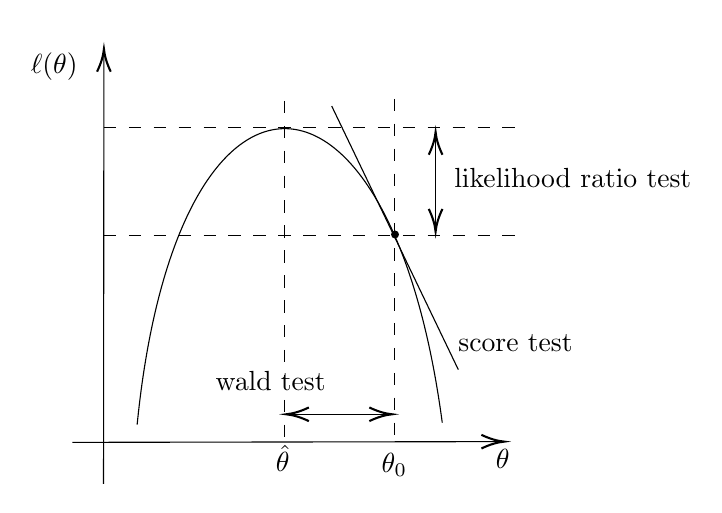
\begin{tikzpicture}[x=0.75pt,y=0.75pt,yscale=-1,xscale=1]
    %uncomment if require: \path (0,300); %set diagram left start at 0, and has height of 300
    
    %Straight Lines [id:da05901855388064847] 
    \draw    (116.28,209.29) -- (322.28,208.93) ;
    \draw [shift={(324.28,208.93)}, rotate = 179.9] [color={rgb, 255:red, 0; green, 0; blue, 0 }  ][line width=0.75]    (10.93,-3.29) .. controls (6.95,-1.4) and (3.31,-0.3) .. (0,0) .. controls (3.31,0.3) and (6.95,1.4) .. (10.93,3.29)   ;
    %Straight Lines [id:da6809814504013212] 
    \draw    (131.28,229.29) -- (131.46,21.76) ;
    \draw [shift={(131.47,19.76)}, rotate = 90.05] [color={rgb, 255:red, 0; green, 0; blue, 0 }  ][line width=0.75]    (10.93,-3.29) .. controls (6.95,-1.4) and (3.31,-0.3) .. (0,0) .. controls (3.31,0.3) and (6.95,1.4) .. (10.93,3.29)   ;
    %Curve Lines [id:da35148800734702434] 
    \draw    (147.47,200.76) .. controls (166.47,9.76) and (269.47,11.76) .. (294.47,199.76) ;
    %Straight Lines [id:da0191225421830008] 
    \draw  [dash pattern={on 4.5pt off 4.5pt}]  (131.47,109.76) -- (331.27,109.76) ;
    %Straight Lines [id:da3881687285855122] 
    \draw  [dash pattern={on 4.5pt off 4.5pt}]  (218.47,44.76) -- (218.47,209.76) ;
    %Straight Lines [id:da9966156097394681] 
    \draw  [dash pattern={on 4.5pt off 4.5pt}]  (271.47,43.76) -- (271.47,208.76) ;
    %Shape: Circle [id:dp6465475156127207] 
    \draw  [fill={rgb, 255:red, 0; green, 0; blue, 0 }  ,fill opacity=1 ] (270.09,109.13) .. controls (270.09,108.23) and (270.82,107.5) .. (271.72,107.5) .. controls (272.62,107.5) and (273.35,108.23) .. (273.35,109.13) .. controls (273.35,110.03) and (272.62,110.76) .. (271.72,110.76) .. controls (270.82,110.76) and (270.09,110.03) .. (270.09,109.13) -- cycle ;
    %Straight Lines [id:da0777384523122382] 
    \draw  [dash pattern={on 4.5pt off 4.5pt}]  (131.47,57.76) -- (331.27,57.76) ;
    %Straight Lines [id:da9382893328394419] 
    \draw    (241.22,47.26) -- (302.22,174.26) ;
    %Straight Lines [id:da5039040124170437] 
    \draw    (221.27,195.76) -- (268.27,195.76) ;
    \draw [shift={(270.27,195.76)}, rotate = 180] [color={rgb, 255:red, 0; green, 0; blue, 0 }  ][line width=0.75]    (10.93,-3.29) .. controls (6.95,-1.4) and (3.31,-0.3) .. (0,0) .. controls (3.31,0.3) and (6.95,1.4) .. (10.93,3.29)   ;
    \draw [shift={(219.27,195.76)}, rotate = 0] [color={rgb, 255:red, 0; green, 0; blue, 0 }  ][line width=0.75]    (10.93,-3.29) .. controls (6.95,-1.4) and (3.31,-0.3) .. (0,0) .. controls (3.31,0.3) and (6.95,1.4) .. (10.93,3.29)   ;
    %Straight Lines [id:da9886798109865442] 
    \draw    (291.27,61.76) -- (291.27,105.76) ;
    \draw [shift={(291.27,107.76)}, rotate = 270] [color={rgb, 255:red, 0; green, 0; blue, 0 }  ][line width=0.75]    (10.93,-3.29) .. controls (6.95,-1.4) and (3.31,-0.3) .. (0,0) .. controls (3.31,0.3) and (6.95,1.4) .. (10.93,3.29)   ;
    \draw [shift={(291.27,59.76)}, rotate = 90] [color={rgb, 255:red, 0; green, 0; blue, 0 }  ][line width=0.75]    (10.93,-3.29) .. controls (6.95,-1.4) and (3.31,-0.3) .. (0,0) .. controls (3.31,0.3) and (6.95,1.4) .. (10.93,3.29)   ;
    
    % Text Node
    \draw (213,209.4) node [anchor=north west][inner sep=0.75pt]    {$\hat{\theta }$};
    % Text Node
    \draw (264,213.4) node [anchor=north west][inner sep=0.75pt]    {$\theta _{0}$};
    % Text Node
    \draw (95,20.4) node [anchor=north west][inner sep=0.75pt]    {$\ell ( \theta )$};
    % Text Node
    \draw (319,211.4) node [anchor=north west][inner sep=0.75pt]    {$\theta $};
    % Text Node
    \draw (301,156) node [anchor=north west][inner sep=0.75pt]   [align=left] {score test};
    % Text Node
    \draw (184,174) node [anchor=north west][inner sep=0.75pt]   [align=left] {wald test};
    % Text Node
    \draw (299,76) node [anchor=north west][inner sep=0.75pt]   [align=left] {likelihood ratio test};
    
    
    \end{tikzpicture}
    \caption{Illustration of Tests on $ \ell(\theta ) $-$ \theta  $ Plot}
    \label{}
\end{figure}



\subsubsection{Non-Parametric Estimation to Survival Function}
In this part we only focus on right censor data $ (\tilde{T}_i,\delta _i) $, $ \delta _i=0 $ for right censoring.

\begin{point}
    Kaplan-Meier Estimator\index{KM Estimator (Kaplan-Meier Estimator)}
\end{point}

Idea of KM Estimator: Separate time into segments by censor/event time $ t_i $, and decompose survival function into products of hazard within segments, using \autoref{EqaSurvivalFunctionDecomposition} which is:
\begin{align}
    \hat{S}(t)=\hat{\mathbb{P}}(T>t)=&\prod_{t_i\leq t}\hat{\mathbb{P}}\left( T>t_i |T>t_{i-1}  \right) \\
    =&\hat{\mathbb{P}}\left( T>t|T>t_i \right)  \prod_{t_i\leq t}\left[1- \hat{\mathbb{P}}\left( t_{i}\geq T>t_{i-1} |T>t_{i-1}\right) \right]\\
    =&\left(1-\hat{\lambda }(t_i)\right)\prod_{t_i\leq t}\left(1-\hat{\lambda }(t_{i-1})\right)\\
    =&\prod_{t_i\leq t}\left[1-\hat{\lambda }(t_i)\right]
\end{align}

where $ \hat{\lambda }(t_i) $ are relatively easy to estimate with censoring considered. $ r_i $ for \# at risk: not censored/event till $ t_i $, $ d_i $ for \# event (death). We can model $ \hat{\lambda }_i $ as
\begin{equation}
    d_i\big|r_i \sim B(r_i,\lambda _i)\xrightarrow[]{\mathscr{L}} N(r_i\lambda _i,r_i\lambda _i(1-\lambda _i))
\end{equation}

and obtain the MLE estimation of $ \hat{\lambda }_i|r_i,d_i $\footnote{Here we use the $ \Delta  $ method for estimating the variance of function of r.v.: if $ X\sim f(\mu ,\sigma ^2) $:
\begin{align}
    g(X)\approx g(\mu )+g'(\mu )(X-\mu )\Rightarrow var(g(X))\approx [g'(\mu )]^2var(X)\leftarrow [g'(X)]^2var(X)
\end{align}}

\begin{align}
    \hat{\lambda }_i=&\dfrac{d_i}{r_i}\\
    var(\hat{\lambda }_i)=&var(\dfrac{d_i}{r_i})=\dfrac{\hat{\lambda }_i(1-\hat{\lambda }_i)}{r_i}\\
    \hat{S}(t)=&\prod_{t_i\leq t}\left[1-\hat{\lambda }(t_i)\right]=\prod_{t_i\leq t}\left[1-\dfrac{d_i}{r_i}\right]\tag{KM Estimator}\\
    var(\hat{S}(t))=&var\left\{ \exp\left[ \log\hat{S(t)} \right] \right\}\\
    \approx&[\hat{S}(t)]^2var\left[\log \hat{S}(t)\right]\\
    =&[\hat{S}(t)]^2\sum_{t_i\leq t}var\left[\log (1-\hat{\lambda }_i) \right]\\
    =&[\hat{S}(t)]^2\sum_{t_i\leq t}\dfrac{1}{(1-\hat{\lambda }_i)^2}var(\hat{\lambda }_i)\\
    =&[\hat{S}(t)]^2\sum_{t_i\leq t}\dfrac{d_i}{r_i(r_i-d_i)}\tag{Greenwood' Formula}\\
    =&[\hat{S}(t)]^2var(\hat{\Lambda }(t))
\end{align}

Interval Estimation of $ \hat{S}(t) $ can be conducted using pointwise interval/confidence band:
\begin{itemize}[topsep=2pt,itemsep=0pt]
    \item Plain pointwise approach:
    \begin{equation}
        \hat{S}(t)\pm N_{1-\frac{\alpha }{2}}\sigma [\hat{S}(t)] 
    \end{equation}
    \item Log-Log pointwise approach (\lstinline|R.| default): using $ \hat{L}(t)=\log\left[-\log \hat{S}(t)\right]=\log\left[\hat{\Lambda }(t)\right] $
    \begin{equation}
         \hat{S}(t)\times e^{\pm N_{1-\frac{\alpha }{2}}\sigma (\hat{L }(t))}
    \end{equation}
    where 
    \begin{equation}
        \sigma (\hat{L }(t))=\sqrt[]{\dfrac{1}{[\log \hat{S}(t)]^2}} \sum_{t_i\leq t}\dfrac{d_i}{r_i(r_i-d_i)}
    \end{equation}
    \item EP confidence band approach
    \item HW confidence band approach
\end{itemize}

Estimator of mean survival time:
\begin{align}
    \hat{\mu }_\tau=&\int _0^\tau \hat{S}(t) \,\mathrm{d}t\\
    var(\hat{\mu }_\tau)=&\sum_{t_i}\left[\int _{t_i}^\tau \hat{S}(t) \,\mathrm{d}t\right]^2\dfrac{d_i}{r_i(r_i-d_i)}
\end{align}
    
\begin{point}
    Nelson-Aalen Estimator\index{NA Estimator (Nelson-Aalen Estimator)}
\end{point}

Idea of NA Estimator: estimate $ \hat{\Lambda }(t) $ first, then obtain Fleming-Harrington Estimator $ \hat{S}_{FH}(t)=e^{-\hat{\Lambda }(t)} $\index{FH Estimator (Fleming-Harrington Estimator)}:
\begin{align}
    \hat{\Lambda }(t)=&\sum_{t_i\leq t}\hat{\lambda }(t_i)=\sum_{t_i\leq t}\dfrac{d_i}{r_i}\\
    var(\hat{\Lambda }(t))=&\sum_{t_i\leq t}\dfrac{d_i(r_i-d_i)}{r_i^2(r_i-1)}\\
    \hat{S}_{FH}(t)=&\exp\left[ -\hat{\Lambda }(t) \right]
\end{align}

\begin{point}
    Survival Function of Life Table
\end{point}

A key difference of survival data of life table is that we cannot know the exact event time/censor time, locating in $ [t_{i-1},t_i) $, in this case we usually estimate $ d_i,\,r_i $ using
\begin{align}
    d_i'=&d_i\\
    r_i'=&r_i-\dfrac{c_i}{2}
\end{align}
where $ c_i $ is \# censor in $ [t_i,t_{i+1}) $, $ r_i $ is \# censoring at the begeinning of interval, i.e. $ t_{i-1} $. And construct KM/NA estimator:
\begin{align}
    \hat{S}_{KM}(t)=&\prod_{t_i\leq t}\left( 1-\dfrac{d_i}{r_i'} \right)\\
    var(\hat{S}_{KM}(t))=&\left[\hat{S}_{KM}(t)\right]^2\sum_{t_i\leq t}\dfrac{d_i}{r_i'(r_i'-d_i)}\\
    \hat{\lambda }(t_{\mathrm{mid\,}i })=&=\dfrac{\hat{f}(t_i)}{\hat{S}(t_i)}= \dfrac{d_i}{(t_{i}-t_{i-1})(r_i'-\frac{d_i}{2})}=\dfrac{d_i}{(t_{i}-t_{i-1})(r_i-\frac{c_i+d_i}{2})}
\end{align}

    where $ \mathrm{mid}\,i  $ means the mid point of $ [t_{i-1},t_{i}) $, i.e. $ \dfrac{t_{i-1}+t_{i}}{2} $


\subsubsection{Hypothesis Testing to Group Comparison}\label{SubSubSectionSurvivalAnalysisGroupComparison}
Key focus: how to judge the difference between two survival function $ S_1(t),\,S_2(t) $, or even when there are more than two groups.

\begin{point}
    Mantel-Haenszel Logrank Test\index{Mantel-Haenszel Logrank Test}
\end{point}\footnote{Note: Log means `time record' here, rather than logarithm.}

Idea of logrank test: adapt contingency table to censor table
\begin{table}[H]
    \centering
    \renewcommand\arraystretch{1}
    \caption{$ 2\times 2 $ contingency table}
    \begin{tabular}{cccc}
        \hline
        \hline
        &\multicolumn{2}{c}{Event $ \delta  $}&\\
        \cline{2-3}
        Group&Yes(1)&No(0)&Total\\
        \hline
        $ 0 $&$ d_0 $&$ r_0-d_0 $&$ r_0 $\\
        $ 1 $&$ d_1 $&$ r_1-d_1 $&$ r_1 $\\
        \hline
        Total&$ d $&$ r-d $&$ r $\\
        \hline
        \hline
    \end{tabular}
    \label{}
\end{table}

\begin{itemize}[topsep=2pt,itemsep=0pt]
    \item Recap: Pearson's $ \chi^2 $ test: assign $ n $ sample into $ k $ groups, and conduct test on $ p_i $, $ i=1,2,\ldots,k $, denote that $ v_i $ samples are assigned to the $ i^\mathrm{th}  $ groups, then
    \begin{equation}
        K_n=\sum_{i=1}^k\dfrac{(v_i-np_i)^2}{np_i}\xrightarrow[]{\mathscr{L}} \chi^2_{df}
    \end{equation}

    In the above example, $ df=k-1 $. In $ 2\times 2 $ contingency table, $ df=1 $ because we assume $ d,r,r_0,r_1 $ are fixed. Pearson's $ \chi^2 $ statistics for $ 2\times 2 $ contingency table:
    \begin{align}
        \chi^2_P=&\sum_{4\text{ grids}}\dfrac{(\mathrm{obs}-\mathrm{expe})^2}{\mathrm{expe} }\\
        =&\dfrac{(d_0-r_0\frac{d}{r})^2}{r_0\frac{d}{r}}+\mathrm{etc}\\
        =&\dfrac{\left[ d_0-r_0\frac{d}{r} \right]^2}{r_0r_1d(r-d)\big/ r^3} \sim \chi^2_1
    \end{align}
    \item Recap: Mental-Haenszel test, based on the Hypergeometric distribution that \index{MH Test (Mental-Haenszel Test)}
    \begin{equation}
        d_0 \sim H(r_0,d,r)\Rightarrow \begin{cases}
            \mathbb{E}\left( d_0 \right)= r_0\dfrac{d}{r}\\
            var(d_0)=\dfrac{r_0r_1d(r-d)}{r^2(r_0-1)}
        \end{cases} ,\quad d_1,r_0-d_0,r_1-d_1 \,\mathrm{similar} 
    \end{equation}

    and construct
    \begin{equation}
        \chi^2_{MH}=\dfrac{\left(\sum_{4\text{ grids}}\mathrm{obs}-\mathbb{E}\left( \mathrm{obs}  \right)\right)^2  }{\sum_{4\text{ grids}} var(\mathrm{obs} )}=\dfrac{\left[ d_0-r_0\frac{d}{r} \right]^2}{\frac{r_0r_1d(r-d)}{r^2(r-1)}}\sim \chi^2_1
    \end{equation}
        
    $ \chi^2_{{MH}} $ and $ \chi^2_{P} $ are equal for lare $ r $.
    \begin{equation}
        \chi^2_{MH}=\dfrac{r-1}{r}\chi^2_P 
    \end{equation}

    \item Cochran-Mantel-Haenszel log-rank test\index{CMH Test (Cochran-Mantel-Haenszel Test)}
    
    For survival data $ t_1,t_2,\ldots,t_K $, we can construct a contingency table $ \mathcal{C}_i $ at each time, and test on the $ K\times 2\times 2 $ contingency table sequence:

    \begin{table}[H]
        \centering
        \renewcommand\arraystretch{1}
        \caption{$ 2\times 2 $ contingency table, $ j=1,2,\ldots,K $}
        \begin{tabular}{cccc}
            \hline
            \hline
            &\multicolumn{2}{c}{Event $ \delta  $}&\\
            \cline{2-3}
            Group&Yes(1)&No(0)&Total\\
            \hline
            $ 0 $&$ d_{0j} $&$ r_{0j}-d_{0j} $&$ r_{0j} $\\
            $ 1 $&$ d_{1j} $&$ r_{1j}-d_{1j} $&$ r_{1j} $\\
            \hline
            Total&$ d_j $&$ r_j-d_j $&$ r_j $\\
            \hline
            \hline
        \end{tabular}
        \label{}
    \end{table}

    and get the CMH statistics for testing $ H_0:\theta _{t_1}=\theta _{t_2}=\ldots =\theta _{t_K} =1$, $ \theta  $ for odds ratio between group 0/1.
    \begin{equation}
        \chi^2 _{CMH}=\dfrac{\left[ \sum_{j=1}^K (d_{0j}-r_{0j}\frac{d_j}{r_j}) \right]^2 }{\sum_{j=1}^K \frac{r_{0j}r_{1j}d_j(r_j-d_j)}{r_j^2(r_j-1)}}\sim \chi^2_1
    \end{equation}

    where the $ K $ contingency tables are treated independent, but they are still ordinal beacuse $ r_{j} $ contains information of history $ d_{t_i<t_j},\, c_{t_i<t_j} $
\end{itemize}

Properties \& Special Cases \& Extension of CMH logrank test:
\begin{itemize}[topsep=2pt,itemsep=0pt]
    \item No tied death $ d_j=1 $:
    \begin{equation}\label{EqaCMHTest}
        \chi^2 _{CMH}=\dfrac{\left[ \sum_{j=1}^K (d_{0j}-r_{0j}\frac{d_j}{r_j}) \right]^2 }{\sum_{j=1}^K \frac{r_{0j}r_{1j}d_j(r_j-d_j)}{r_j^2(r_j-1)}}= \dfrac{\left[ \sum_{j=1}^K (d_{0j}-r_{0j}\frac{d_j}{r_j}) \right]^2 }{\sum_{j=1}^K \frac{r_{0j}r_{1j}}{r_j^2}} \sim \chi^2_1,\quad d_{0j}\in\{0,1\}
    \end{equation}
    \item Intuition of $ \mathrm{obs}-\mathbb{E}\left( \mathrm{obs}  \right)   $:
    \begin{align}
        \mathrm{obs}-\mathbb{E}\left( \mathrm{obs}  \right) \approx& d_{0j}-d_j\dfrac{r_{0j}}{r_{j}}\\
        =&\dfrac{r_{0j}r_{1j}}{r_j}\left(\hat{\lambda }_{0j}-\hat{\lambda }_{1j}\right)
    \end{align}
    \item Attach weight $ w_i\geq 0 $, $ i=1,2,\ldots ,K $ to $ \mathcal{C}_i $:
    \begin{equation}
        \chi^2_{CMH,w}=\dfrac{\left[ \sum_{j=1}^K w_j(d_{0j}-r_{0j}\frac{d_j}{r_j}) \right]^2 }{\sum_{j=1}^K w_j^2\frac{r_{0j}r_{1j}d_j(r_j-d_j)}{r_j^2(r_j-1)}}\sim \chi^2_1
    \end{equation}
    
    bu choosing differnet kinds of weight $ \vec{w} $ we could get variants of CMH test.
    \begin{itemize}[topsep=2pt,itemsep=0pt]
        \item $ w_i=1 $ for log-rank test. Focus more on difference at large $ t $
        \item $ w_i=r_i $ for generalized Wilcoxon rank sum test.  Focus more on difference at small $ t $.
    \end{itemize}
    
    Note: weighted log-rank test should be used when \textbf{no cross}  btw. $ S_1(t) $ and $ S_2(t) $. Kink-of-Weight to choose depends on $ H_1 $.
        
    
\end{itemize}



\begin{point}
    Generalized Wilcoxon Rank Sum Test\index{Wilcoxon Two-Sample Rank Sum Test}
\end{point}

\begin{itemize}[topsep=2pt,itemsep=0pt]
    \item Wilcoxon Two-Sample Rank Sum Test: Knowledge of Wilcoxon two-sample rank sum test see \autoref{SubSectionIntroToNonParametricHypothesisTesting}. Recap: to test the distribution difference of $ \vec{X}=(X_{1},X_{2},\ldots,X_{n})  $ and $ \vec{Y}=(Y_{1},Y_{2},\ldots,Y_{m})  $, we mix them together  and rank as $ \vec{Z}=(Z_{(1)},Z_{(2)},\ldots,Z_{(m+n)})$. Rank of $ X_i $:
    \begin{align}
        R_{i}\equiv &\mathrm{rank}(X_i)\text{ in } \vec{Z},\quad i=1,2,\ldots,n  \\
        R\equiv &\sum_{i=1}^nR_i
    \end{align}
        
    A rank sum statistic to test:
    \begin{align}
        &\dfrac{R-\mathbb{E}\left( R \right)}{\sqrt[]{var(R)}}\sim N(0,1)\\
        &\begin{cases}
            \mathbb{E}\left( R \right) =\dfrac{n(m+n+1)}{2}\\
            var(R)=\dfrac{mn(m+n+1)}{12}
        \end{cases}
    \end{align}

    Rank sum statistic can be written in a Mann-Whitney form that can be generalized:\index{Mann-Whitney Form}
    \begin{align}
        U_{ij}=&U(X_i,Y_j)\equiv\begin{cases}
            +1&,\text{case } X_i>Y_j\\
            0&,\text{case } X_i=Y_j\\
            -1&,\text{case }X_i<Y_j
        \end{cases},\qquad U=\sum_{i,j}^{n,m}U_{ij}\\
        R=&\dfrac{n(m+n+1)}{2}+\dfrac{U}{2}
    \end{align}

\item Mann-Whitney-Wilcoxon rank sum test for censored data: 

    Notation: we still mix $ X=\{(\tilde{t}_{1i},\delta _{1i})\}_{i=1}^n $ and $ Y=\{(\tilde{t}_{2j},\delta _{2j})\}_{j=1}^m $ to get:
    \begin{equation}
        Z_\mathrm{mix}=\left\{ (\tilde{t}_i,\delta _i) \right\}_{i=1}^{m+n}  
    \end{equation}
    and the Mann-Whitney form for $ Z_\mathrm{mix}  $:
    \begin{align}
        U_{ij}=&U(Z_i,Z_j)  \equiv\begin{cases}
            +1&,\text{case } \tilde{t}_i>\tilde{t}_j,\, \delta _j=1\\
            0&,\text{case }  \tilde{t}_i=\tilde{t}_j \text{ or } \delta _j=0\\
            -1&,\text{case } \tilde{t}_i<\tilde{t}_j,\, \delta _j=1
        \end{cases},\quad i=1,2,\ldots ,m+n.\, j=1,2,\ldots ,m+n.
    \end{align}
         
    and the Extended Wilcoxon rank sum statistic:
    \begin{equation}
         W=\sum_{i\text{ if }Z_i\in X}^{m+n}\sum_{j=1}^{m+n}U_{ij}
    \end{equation}

    Under $ H_0: X\sim Y $, distribution features
    \begin{align}
        \mathbb{E}\left( W \right) =&0\\
        \hat{var}(W)=&\dfrac{mn}{(m+n)(m+n-1)}\sum_{i=1}^{m+n}\left(\sum_{j=1}^{m+n}U_{ij}\right)^2
    \end{align}

    \begin{itemize}[topsep=2pt,itemsep=0pt]
        \item choose $ w_i=r_i $ in weighted log-rank test, and nominator becomes
        \begin{align}
            \sum_{j=1}^Kr_j(d_{0j}-r_{0j}\dfrac{d_j}{r_j})=&\sum_{j=1}^K\left[ (r_{1j}-d_{1j})d_{0j}-(r_{0j}-d_{0j})d_{1j} \right]\\
            =&\sum_{j=1}^K\left[ \#_{Y>t_j}\times \#_{X=t_j}-\#_{X>t_j}\times \#_{Y=t_j}  \right]\\
            =&\#_{Y>X}-\#_{Y<X}\\
            =&-W
        \end{align}
        in which $ \chi^2_{w_i=r_i,CMH} $ test is the same as generalized Wilcoxon rank sum test.
        
        
    \end{itemize}
    
        
\end{itemize}

\subsection{Survival Model with Covariants} 

To research on the dependence of $ T $ with regard to covariants $ z $. Survival data with covariants: $ X=(\tilde{t}_i,\delta _i,z_i) $

\subsubsection{Cox's Proportion Hazard Model}
Basic assumption on dependence form: $ T $ hazard part and covariants part are Separatable:\index{PH Model (Cox's Proportion Hazard Model)}
\begin{equation}
    \lambda (t|z)=\lambda _0(t)g(z)\Leftrightarrow S(t|z)=\left[S_0(t)\right]^{g(z)},\quad S_0(t)=e^{-\int _0^t\lambda _0(\tau) \,\mathrm{d}\tau}
\end{equation}

further a linear form $ g(z)=\beta ^Tz $ is used;
\begin{equation}
     \lambda (t|z)=\lambda _0(t)\exp\left[ \beta ^Tz \right]
\end{equation}

Basic Assumptions of Cox's PH Model:
\begin{itemize}[topsep=2pt,itemsep=0pt]
    \item constant regression coefficient $ \beta  $;
    \item linear dependent of covariants $ \beta 'z $;
    \item exponential link function $ e^\cdot $
\end{itemize}

    

in this proportion hazard model, the ratio of hazard only depend on $ \beta  $:
\begin{equation}
    \log\left\{ \dfrac{\lambda _{z_i}(t)}{\lambda _0(t)} \right\}=\beta ^Tz_i\parallel t 
\end{equation}

The unknown components are $ \lambda _0(t),\beta  $, where the $ \lambda _0(t) $ lies in the $ dim\to\infty $ space, and causes difficulty in conducting inference. Solution: decompose full likelihood into two parts, in which one of them, \textbf{Partial Likelihood} is only function of $ \beta  $:\index{Partial Likelihood}
\begin{align}
    L(\beta ,\lambda _0(\cdot);X)=&\prod_{i}\left[ \left( \lambda _0(t_i)e^{\beta ^Tz_i} \right)^\delta _i\left( e^{-\int _{0}^{t_i}\lambda _0(\tau) \,\mathrm{d}\tau} \right)^{e^{\beta ^Tz_i}} \right]\\
    =&L_{PH}(\beta ;X)L_{res}(\beta ,\lambda _0;X)
\end{align}

and we could focus on $ L_{PH} $ for further inference.

Note: the feasibility of partial likelihood comes from the form of proportion hazard.

\begin{point}
    Partial Likelihood without Tie
\end{point}

\textit{Derivation:} First we assert $ t_i $ in ascending order and without tie: $ t_1<t_2<\ldots <t_n $, and we use an discrete estimated form of $ \lambda _0(t_i)=\lambda _i $
\begin{equation}
    \int _0^{t_i}\lambda _0(\tau) \,\mathrm{d}\tau \approx \sum_{j=1}^i\lambda _j
\end{equation}
then we could use a trick to reformulate $ \ell(\beta ,\lambda _1,\ldots,\lambda _n;X) $ as\footnote{\newcommand{\blue}{\color{blue}}\newcommand{\brown}{\color{brown}}
Illustration for $ \blue\displaystyle\sum_{i=1}^n\lambda _i\sum_{j=i}^ne^{\beta 'z_j}=\sum_{i=1}^n\sum_{j=1}^i\lambda _je^{\beta 'z_i} $
\begin{equation}\begin{pNiceMatrix}[last-row,last-col,nullify-dots,xdots/line-style={dashed,blue}]

\lambda _1e^{\beta 'z_1}&&&&&\brown\leftarrow\sum_{j=1}^1\lambda _je^{\beta 'z_1}\\
\lambda _1e^{\beta 'z_2}&\lambda _2e^{\beta 'z_2}&&&&\brown\leftarrow\sum_{j=1}^2\lambda _je^{\beta 'z_2}\\
\lambda _1e^{\beta 'z_3}&\lambda _2e^{\beta 'z_3}&\lambda _3e^{\beta 'z_3}&&&\brown\leftarrow\sum_{j=1}^3\lambda _je^{\beta 'z_3}  \\
\vdots&\vdots&\vdots&\ddots&&\brown\leftarrow\vdots\\
\lambda _1e^{\beta 'z_n}&\lambda _2e^{\beta 'z_n}&\lambda _3e^{\beta 'z_n}&\cdots&\lambda _ne^{\beta 'z_n}&\brown\leftarrow\sum_{j=1}^n\lambda _je^{\beta 'z_n}\\
\brown\overset{\uparrow}{\lambda _1\sum_{j=1}^ne^{\beta 'z_j}}&\brown\overset{\uparrow}{\lambda _2\sum_{j=2}^ne^{\beta 'z_j}}&\brown\overset{\uparrow}{\lambda _3\sum_{j=3}^ne^{\beta 'z_j}}&\brown\overset{\uparrow}{\cdots}&\brown\overset{\uparrow}{\lambda _n\sum_{j=n}^ne^{\beta 'z_j}}&\blue\sum_{i=1}^n\lambda _i\sum_{j=i}^ne^{\beta 'z_j}=\sum_{i=1}^n\sum_{j=1}^i\lambda _je^{\beta 'z_i}
\end{pNiceMatrix}\end{equation}
}

\begin{align}
    \ell(\beta ,\lambda _1,\ldots,\lambda _n)=&\sum_{i=1}^n\left\{ \delta _i(\log\lambda _i+\beta 'z_i)-{\color{blue}\sum_{j=1}^i\lambda _je^{\beta 'z_i}} \right\}\\
    =&\sum_{i=1}^n\left\{ \delta _i(\log\lambda _i+\beta 'z_i)-{\color{blue}\lambda _i\sum_{j=i}^ne^{\beta 'z_j}} \right\}
\end{align}

and use MLE with regard to $ \lambda _i $ to get an estimate to $ \lambda _i $: 
\begin{equation}
    \dfrac{\partial^{} \ell(\beta ,\lambda _1,\ldots,\lambda _n)}{\partial \lambda _i^{}}=0\Rightarrow \lambda _i(\beta )=\dfrac{\delta _i}{\sum_{j=1}^ne^{\beta 'z_j}} \quad \forall i
\end{equation}

then we could get the partial likelihood
\begin{align}
    L(\beta ,\lambda _1(\beta ),\ldots,\lambda _n(\beta ))=&\prod_{i=1}^n\lambda _i(\beta )^{\delta _i}e^{\delta _i\beta 'z_i}e^{-\sum_{j=1}^ne^{\beta 'z_i}}\\
    =&e^{-\sum_i\delta _i}\prod_{i=1}^n\left( \dfrac{e^{\beta 'z_i}}{\sum_{j:t_j\geq t_i}e^{\beta 'z_j}} \right)^{\delta _i}\\
    PL(\beta )\equiv&\prod_{i=1}^n\left( \dfrac{e^{\beta 'z_i}}{\sum_{j:t_j\geq t_i}e^{\beta 'z_j}} \right)^{\delta_i}\\
    P\ell=&\sum_{i=1}^n\delta _i\left[ \beta 'z_i-\log\left(\sum_{j:t_j\geq t_i}e^{\beta 'z_j}\right) \right]\\
    U(\beta )=&\sum_{i=1}^n\delta _i\left[ z_i-\dfrac{\sum_{j:t_j\geq t_i}z_je^{\beta 'z_j}}{\sum_{j:t_j\geq t_i}e^{\beta 'z_j}} \right]\\
    J(\beta )=&\sum_{i=1}^n\delta _i\left[ \sum_{j:t_j\geq t_i}^n \dfrac{e^{\beta 'z_j}}{\sum_{l:t_l\geq t_j}e^{\beta 'z_l}} \left( z_j-\dfrac{\sum_{l:t_l\geq t_j}z_le^{\beta 'z_l}}{\sum_{l:t_l\geq t_j}e^{\beta 'z_l}} \right)^2 \right]
\end{align}

The above statistics can be use for further inference.
\begin{align}
    &J(\beta _0)^{-1/2}U(\beta _0)\xrightarrow[]{\mathscr{L}} N(0,1)\\
    &(\hat{\beta }-\beta _0)\xrightarrow[]{\mathscr{L}} N(0,J(\hat{\beta })^{-1})\\
    &2(\ell(\hat{\beta })-\ell(\beta))\xrightarrow[]{\mathscr{L}} \chi^2_p
\end{align}

\begin{point}
    Modification for Partial Likelihood with Tie
\end{point}

There are various modification for tied data case. In PL without tie, the $ \dfrac{e^{\beta 'z_i}}{\sum_{j:t_j\geq t_i}e^{\beta 'z_j}} $ term are usually changed to adapt for the case of. Intuition:
\begin{equation}
    \dfrac{e^{\beta 'z_i}}{\sum_{j:t_j\geq t_i}e^{\beta 'z_j}}=\dfrac{\lambda (t_i|z_i)}{\sum_{j:t_j\geq t_i}\lambda (t_j|z_j)}\approx \mathbb{P}\left( i^\mathrm{th} \text{event}|1\text{out of }\# \{j:t_j\geq t_i\}  \right) 
\end{equation}

Notation: $\mathcal{R}_i $ for all datapoints at risk at time $ t_i $, $ \mathcal{D}_i $ for event cases at time $ t_i $, $ \mathcal{D}_i\subset \mathcal{R}_i $
\begin{itemize}[topsep=2pt,itemsep=0pt]
    \item Cox's modification:\indexname{Cox's Modification}
    \begin{equation}
        \mathbb{P}\left( \mathcal{D}_i \text{ events}\Big| |\mathcal{D}_i |\text{out of }\# \{j:t_j\geq t_i\}  \right)=\dfrac{e^{\sum_{l\in\mathcal{D}_i }\beta'z_l }}{\sum_{\text{all possible }|\mathcal{D}_j|=|\mathcal{D}_i | }e^{\sum_{l\in\mathcal{D}_j }\beta'z_j} }
    \end{equation}
    drawback: $ \sim O(|\mathcal{D}_i|!) $ complexity
    \begin{align}
        PL(\beta )=&\prod_{i=1}^n\left\{ \dfrac{e^{\sum_{l\in\mathcal{D}_i}\beta 'z_l}}{\sum_{\text{all possible }|\mathcal{D}_j|=|\mathcal{D}_i|}e^{\sum_{l\in\mathcal{D}_j}}e^{\sum_{l}\in\mathcal{D}_j}\beta 'z_l} \right\} 
    \end{align}
    
    
    \item Breslow's approximation:\index{Breslow's Approximation}
    \begin{equation}
        \mathbb{P}\left( \mathcal{D}_i \text{event}\Big| |\mathcal{D}_i |\text{out of }\# \{j:t_j\geq t_i\}  \right)\approx \dfrac{e^{\sum_{l\in\mathcal{D}_i }\beta'z_l }}{\left(\sum_{l\in\mathcal{R}_i}e^{\beta 'z_l}\right)^{|\mathcal{D}_i|}}
    \end{equation}
    or directly write the PL as
    \begin{equation}
        PL(\beta )=\prod_{i=1}^n \left\{ \prod_{j\in\mathcal{D}_i}\dfrac{e^{\beta 'z_j}}{\sum_{l\in\mathcal{R}_i}e^{\beta 'z_l}} \right\}
    \end{equation}
    \item Efron's approximation: usually better than Breslow's, default method in \lstinline|coxph()|\index{Efron's Approximation}
    \begin{align}
        PL(\beta )=\prod_{i=1}^n\left\{ \dfrac{e^{\sum_{l\in\mathcal{D}_i}\beta 'z_l}}{ \prod_{j=1}^{|\mathcal{D}_i|}\left( \sum_{l\in\mathcal{R}_i}e^{\beta 'z_l}-\frac{j-1}{|\mathcal{D}_i|}\sum_{l\in\mathcal{D}_i}e^{\beta 'z_l} \right) } \right\} 
    \end{align}
    
    
\end{itemize}


\begin{point}
    Extension for Time-Dependent Variable
\end{point}

Model:
\begin{align}
    \begin{cases}
        \lambda (t)=&\lambda _0(t)e^{\beta 'z(t)}\\
        \lambda (t)=&\lambda _0(t)e^{\beta (t) 'z}
    \end{cases}
\end{align}

\begin{point}
    Diagnostic Methods for PH Assumption
\end{point}

\begin{itemize}[topsep=2pt,itemsep=0pt]
    \item $ \log $-$ \log $ plots: for categorical $ z_1 $, $ z_2 $, use relation
    \begin{align}
        \log\left[-\log S(t,z_1)\right] -\log\left[-\log S(t,z_2)\right] =\beta '(z_1-z_2)\independent t
    \end{align}
    
    Plot of $ \log\left[\log \hat{S}(t,z)\right] $ should be 'parallel' curves.
    
    \item Check the coherence bet. observed data v.s. expected data.
    \item Goodness-of-fit using Schoenfeld residuals\indexname{Schoenfeld Residual}
    \begin{align}
        \hat{r}_i=&z_i-\sum_{j\in\mathcal{R}_i}z_k\cdot p(\hat{\beta },z_k)=z_i\bar{z}_i\\
        p(\beta ,z_k):=&\dfrac{e^{\beta 'z_k}}{\sum_{j\in\mathcal{R}_k}e^{\beta 'z_j}} 
    \end{align}
    \item (Generalized) Cox-Snell Residual for overall goodness-of-fit: \index{Cox-Snell Residual}
    
    Recall: for r.v. $ T\sim f(t) $, $ S(t)=\int _t^\infty f(\tau) \,\mathrm{d}\tau $. function of r.v. has distribution:
    \begin{align}
        S(T)\sim U(0,1)\Rightarrow \Lambda (T)\sim \varepsilon (1) 
    \end{align}

    define Cox-Snell Residual:
    \begin{align}
        \hat{\Lambda }(z_i)=-\log \hat{S}(z_i) 
    \end{align}

    the set $ \{\hat{\Lambda }(z_i)\} $ could be viewed as a sample from $ \varepsilon (1) $, we could test on the distribution, e.g. plot the cumulative hazard \textbf{of residual} v.s. residual to check $ \Lambda (e)=e $.
    
    \item Delta-Beta Residual for infulential: \index{Delta-Beta Residual} for $ \beta =(\beta _0=1,\beta _1,\ldots) $, define
    \begin{align}
        \hat{\Delta }_{ij}=\hat{\beta }_j-\hat{\beta }_{j(\wedge i)} 
    \end{align}

    where $ \wedge i $ for estimator with the $ i^\mathrm{th}  $ subject removed. Plot the scatter plot of $ \hat{\Delta }_{ij} $ to locate influential.

    % \item Martingale Residual for non-linearity: \index{Martingale Residual}
\end{itemize}

\begin{point}
    Experiment Design for Log-rank Test under PH Assumption
\end{point}

    Question: how many events are needed for the testing $ H_0:\beta =0\leftrightsquigarrow H_a:\beta =\beta _a $?

    Using log-rank statistics \autoref{EqaCMHTest} in $ z $-test form, under condition 1. no ties $ d_j=0,1 $, 2. $ \beta _a $ is small enough for taylor expansion:\footnote{Proof key: 
    \begin{align}
        d_{0j}\sim B(p_{0j}), \quad  p_{0j}=\dfrac{r_{0j}\lambda _0}{r_{0j}\lambda _0+r_{1j}\lambda _0e^{\beta _a} }
    \end{align}
    
    and at small $ \beta _a $, take approximation $ \theta \approx r_{1j}/r_{j} $
    }
    \begin{align}
        T_{CMH}= \dfrac{\sum_{j=1}^K\left( d_{0j}-r_{oj}\frac{d_j}{r_j} \right)}{\sqrt[]{\sum_{j=1}^K}\frac{r_{0j}r_{1j}d_j(r_j-d_j)}{r_j^2(r_j-1)}}\xrightarrow[]{\mathscr{L}} N(\beta _a\sqrt[]{d\theta (1-\theta )}, 1)
    \end{align}

    where $ d=\sum_{j=1}d_j $, $ \theta  $ is the prevalence of group 1.

    Power of the test: denote $ \gamma  $ for probability of type II error
    \begin{align}
        \mathbb{P}\left( T_{CMH}>N_{\alpha /2}|H_a \right) = 1-\gamma \Rightarrow \mu :=\beta _a\sqrt[]{d\theta (1-\theta )}\approx N_{\alpha /2}+N_\gamma 
    \end{align}

    Minimum number of events:
    \begin{align}
        d=\dfrac{(N_{\alpha /2}+N_\gamma )^2}{\beta _a^2\theta (1-\theta )} 
    \end{align}
    
    
    
    
    
    

    

\subsubsection{Accelerated Failure Time Model}

    Basic form of AFT Model (Accelerated Failure Tome Model)\index{AFT Model (Accelerated Failure Tome Model)} for categorical covariants:
    \begin{align}
        S(t;z=1)=S(\gamma t;z=2)\Leftrightarrow \mathbb{P}\left( T_1>t \right) =\mathbb{P}\left( T_2>\gamma t \right)  
    \end{align}

    Usually we attach some assumptions on function form of $ S(t,z) $, usually take (parameter denoted $ \alpha  $):
\begin{itemize}[topsep=2pt,itemsep=0pt]
    \item Exponential:
    \begin{align}
        S(t)=&e^{-\lambda t},\quad \lambda (t)=\lambda \\
        \Rightarrow &t=-\dfrac{1}{\lambda }\log S(t)\\
        \Rightarrow &\gamma :=e^{\alpha 'z}=\dfrac{1}{\lambda }=e^{-\beta 'z}
    \end{align}

    i.e. Exponential AFT model in which $ \gamma =e^{\alpha 'z} $ is equivalent to PH model with $ \lambda =e^{\beta 'z} $, and $ \beta =-\alpha  $ 
    
    \item Weibull:
    \begin{align}
        S(t)=&e^{-\lambda t^p},\quad \lambda (t)=\lambda pt^{p-1}\\
        \Rightarrow &t=-\dfrac{1}{\lambda ^{1/p}}\log S(t)\\
        \Rightarrow &\gamma :=e^{\alpha 'z}=\dfrac{1}{\lambda ^{1/p}}=e^{-\beta 'z/p}
    \end{align}
    
    i.e. Weibull AFT model with $ \gamma =e^{\alpha 'z} $ is equivalent to PH model with $ \lambda =e^{\beta 'z} $, and $ \beta =-\alpha p $
    
    \item General Case: In different groups $ z $, survivial time 
    \begin{align}
        T_i=&T_0e^{\alpha 'z_i+ \varepsilon _i/p },\quad \varepsilon _i\sim \varepsilon (1)
        S_i(t)=&\mathbb{P}\left( T_i\geq t \right)\\
        =&\mathbb{P}\left( \log T_0 +\alpha 'z_i+\dfrac{\varepsilon _i}{p}\geq  \log t \right)  \\
        =&S_{\varepsilon (1)}\left(p({\log t-\log T_0-\alpha 'z_i})\right)
    \end{align}
    
    
    
    
\end{itemize}


\begin{point}
    AFT Model and PH Model
\end{point}

    An intuition for parameters in AFT model and PH model:
\begin{figure}[H]
    \centering
    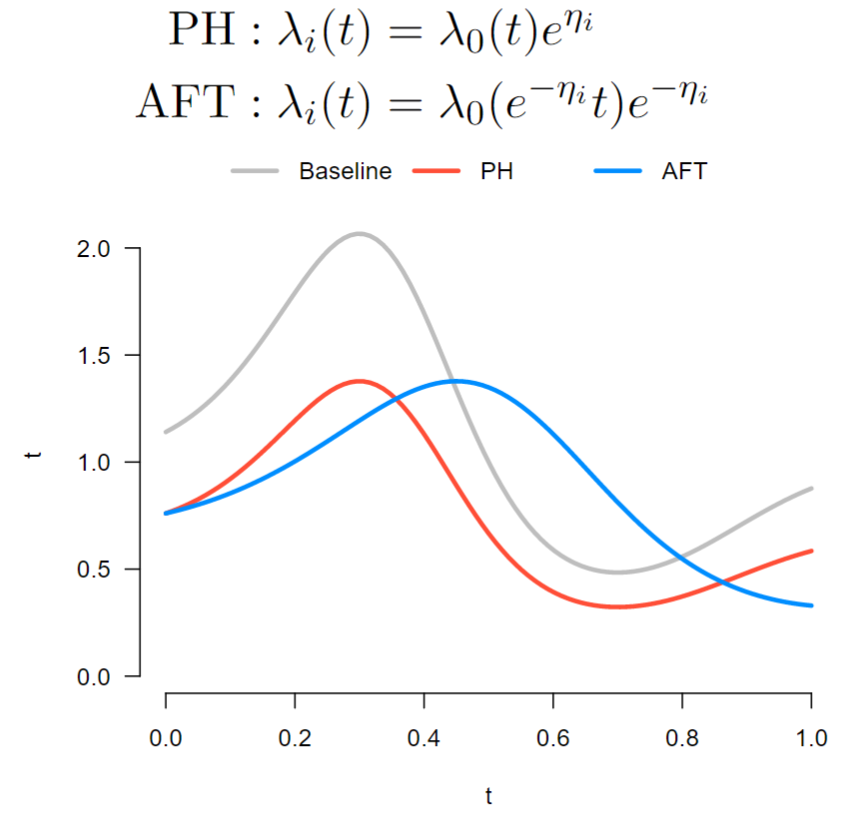
\includegraphics[width=0.45\linewidth]{sections/images/2022-08-19-10-03-10.png}
    \label{}
\end{figure}

    Usually AFT model depends on a parametric model, whlie PH model only depends on the PH assumption.



\begin{rcode}
    An example:
\begin{lstlisting}[language=R]
coxph(formula = Surv(start, stop, event) ~ rx + number + size + factor(enum), data = bladder2)
\end{lstlisting}
\end{rcode}
    
    


    
